\documentclass[a4paper]{article}

%% Language and font encodings
\usepackage[frenchb]{babel}
\usepackage[utf8x]{inputenc}
\usepackage[T1]{fontenc}
\usepackage{minted} %compiler avec la commande -shell-escape
\usepackage{graphicx}
\usepackage{dirtree}

%% Todo List
\usepackage{enumitem,amssymb}
\newlist{todolist}{itemize}{2}
\setlist[todolist]{label=$\square$}
\usepackage{pifont}
\newcommand{\cmark}{\ding{51}}%
\newcommand{\xmark}{\ding{55}}%
\newcommand{\done}{\rlap{$\square$}{\raisebox{2pt}{\large\hspace{1pt}\cmark}}%
\hspace{-2.5pt}}
\newcommand{\wontfix}{\rlap{$\square$}{\large\hspace{1pt}\xmark}}

%% Sets page size and margins
\usepackage[a4paper,top=3cm,bottom=2cm,left=3cm,right=3cm,marginparwidth=1.75cm]{geometry}
\setlength{\parskip}{.5em}

\newcommand{\HRule}{\rule{\linewidth}{0.5mm}}

%-------------------------------------------------------------------------------
% TITLE PAGE
%-------------------------------------------------------------------------------

\begin{document}

\title
{
	\HRule \\ [0.5cm]
	\LARGE \textbf{\uppercase{Projet technologique}}
	\HRule \\ [0.5cm]
}

\date{}

\author
{
	\LARGE{Université de Bordeaux} \\
	\\
        Enzo Peruzzetto \\
        Michel MASSAMIRI\\
        Matthias PAULMIER\\
}

\begin{document}

\null  % Empty line
\nointerlineskip  % No skip for prev line
\vfill
\let\snewpage \newpage
\let\newpage \relax
\maketitle
\let \newpage \snewpage
\vfill
\break % page break
%-------------------------------------------------------------------------------
% Table des matières
%-------------------------------------------------------------------------------

\tableofcontents
\newpage

%-------------------------------------------------------------------------------
% Présentation du projet - Introduction
%-------------------------------------------------------------------------------

\section{Présentation du projet}
	\emph{ Web et base de données : un outil pour les seniors et personnes handicapées}\\

Les collectivités locales, les mairies par exemple, communiquent largement via Internet. Cependant des publics comme les séniors ou les personnes handicapées n'ont pas un accès simple aux informations spécifiques qui les intéressent sur les sites de ces collectivités et il est souhaitable d'enrichir les services qui leur sont proposés sur le web.\\

L'objectif du projet est donc de créer une base d’informations accessible et intuitive permettant aux personnes les moins à l’aise avec l’outil informatique de s'informer et de trouver une réponse à leurs questions. Voici des exemples de fonctionnalités : accès à l’ensemble des services pour les séniors et les personnes handicapées (aides à domicile, soins infirmiers, loisirs,. . . ), visualisation des services disponibles, accès à un espace où les personnes âgées ou leurs familles pourraient poser leurs questions, collecte et partage des propositions de bénévoles (petits travaux, aide aux transports, etc). En pratique, le projet consiste à développer un prototype livrable de site Internet accompagné de sa base de données.

\newpage
%---------------------------------------------------------------------------------
%  Cahier des Charges
%---------------------------------------------------------------------------------
\section{Cahier des Charges}

\subsection{Présentation de l'entreprise}

La mairie de Bègles aimerait mettre en place sur leur site internet une application web permettant aux personnes agées et handicapés de pouvoir obtenir des informations sur certains services.

\subsection{besoins de la mairie}

Mise en ligne d’une base d'informations recensant l’ensemble des services pour les séniors et les personnes handicapées:
\begin{itemize}
\item aides et accompagnement à domicile
\item soins infirmiers
\item partage services
\item loisirs\\
\end{itemize}


Reliée au site internet de la ville, cette base de données permettrait de visualiser les services disponibles.\\

Créer un espace où les personnes âgées ou leurs familles pourraient poser leurs questions.
Créer un espace pour rassembler les propositions des habitants de la commune qui souhaiteraient s’investir dans le bénévolat et notamment aider les plus âgées via des visites de courtoisie, de l’aide aux petits travaux, de l’aides aux transports, etc.

\subsection{objectifs}

Pour répondre à ses besoins, nous avons pensés aux services suivants:

Créer une base d’informations accessible et intuitive permettant aux personnes les moins à l’aise avec l’outil informatique de trouver une réponse à leurs questions.
Créer un outil pour les agents du service leur permettant de répertorier l’offre à destination de ce public et de suivre son évolution dans la commune.\\

\subsection{besoin fonctionnel}


\subsubsection{base de donnée }

Une base de donnée MySQL sera délivré avec le site pour toute la partie de stockage de données. Elle est composée de table MySQL décrit ci-dessous:
\begin{itmesize}
\item Une table de users.
\item Une table de services.
\item Une table de questions.
\item Une table de reponse.
\end{itemsize}

\subsubsection{Une page d'identification }

Cette page sera de la forme d'un formulaire, elle aura les fonctions suivantes:
\begin{itemsize}
\item Une fonction qui permet l'authentification d'un utilisateur.
\item Une fonction qui permet l'inscription d'un utilisateur.
\item Une fonction qui vérifie si les champs sont bien remplis et bien écrit.
\end{itemsize}

\subsubsection{FAQ }

Se service permettra aux utilisateurs de poser et répondre à certaines questions.
Elle aura donc les fonctions suivantes:
\begin{ itemsize }
\item Une fonction permettant de poser une question dans le FAQ.
\item Une fonction permettant de valider la question poser.
\item Une fonction permettant de repondre à la question.
\end{ itemsize}

\subsubsection{Listes des services disponnibles }
Le site web permet d'afficher à tous les utilisateurs de site les services qui sont disponibles dans la base de données.
Ceci dit que le visiteur du site pourrait regarder tous les services mises par l'administrateur du site.

<<<<<<< HEAD
=======
Les informations que les services vont fournir sont les suivants :
\begin{ itemsize }
	\item Le type de service. Exemple : Aide à domicile, Faire les courses, loisir, etc...
	\item Le lieu de l'événement.
	\item La date du service.
	\item Une description courte qui explique le service.
	\item L'auteur de l'annonce (l'organisateur du service).
\end{ itemsize }
\subsubsection{Listes des utilisateurs}

>>>>>>> 4411fe64709b31e569b74cd1d37789b2e5a07d01
\subsubsection{Inscription}

L'inscription se fera sur un formulaire qui regarde au préalable si le client n'est pas déjà inscrit.

\subsubsection{Interface admin}

Cet outil permettra aux administrateurs du site de gérer la suppression, la modification des services, des questions et des réponses, aussi des utilisateurs.
Également, l’administrateur pourrait ajouter des services sur le site.
%(organisation des pages PHP et SQL)
%Décrire les pages accessibles, comment elles s’organisent (classes PHP ?), quelle est la bdd associée:
%Publique Services disponibles
%Admin Services disponibles
%Publique Questions aux agents
%Admin Questions aux agents
%Publique Propositions (modéré)
%Admin Propositions
%modularite cote admin
\newpage
%---------------------------------------------------------------------------------
% Descriptif de la base de donnée
%---------------------------------------------------------------------------------
\section{Descriptif de la base de donnée}

\begin{figure}[!hp]
\center
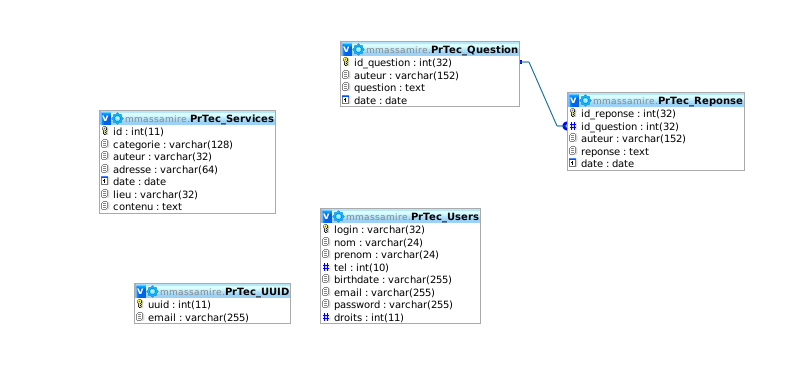
\includegraphics[width= 15cm]{bdd.png}
\caption{Base de donnée du site}
\end{figure}

Pour le service FAQ, les tables de la base relié a se service sont les tables PrTec\_Question et PrTec\_Reponse. Comme on peut le voir sur l'image ci-dessus la table question et réponse sont liées, le id\_question de la table réponse corresponds à l'identifiant d'une question stockée dans la table question.

%-------------------------------------------------------------------------------
% Le service d'inscription et d'identification
%-------------------------------------------------------------------------------
\section{Gestion des utilisateurs}
Pour la gestion des utilisateurs il y a deux fonctionnalités
principales. Celles-ci ont été adaptés de code produit en TD lors du
premier semestre.

\subsection{Inscription}
Pour l'inscription, l'utilisteur remplit les champs qui lui sont
demandés avec ses informations. A la validation du formulaire, un
identifiant unique (UUID dans la base de données) est créé. Il permet
d'identifié le client. Un email est envoyé au client contenant une URL
unique avec cet UUID (fonction neutralisée pour ne pas encombrer les
serveurs du cremi mais réactivable simplement dans le code).

\subsection{Identification}
Un utilisateur inscrit peut alors s'identifier. La page principale du
site sert cette fonctionnalité. Lorsque l'utilisateur saisie ses
identifiants, on vérifie sa présence dans la base de données (le login
est unique et sert de clé primaire pour la table Users). Si il existe,
on récupère ses données pour les mettre dans la session et on lui
donne accès aux fonctionnalités du site.

Lors d
%-------------------------------------------------------------------------------
% Le service liste de services
%-------------------------------------------------------------------------------
\section{Liste des services}

Cette fonctionnalité a été réalisé par les ‘controller/services.php’, ‘model/services’ et ‘view/listServices.php’.

Le ‘controller/services.php’ est le fichier principal qui contrôle l’échange entre le ‘model’ et la ‘view’. Donc, si l’utilisateur veut regarder la liste des services, il appelle le ‘controller/services.php’, ce dernier appellera le ‘model/services.php’. Ensuite, le ‘model’ contient toutes les fonctions qui seront utiles pour afficher, insérer, modifier ou bien supprimer un service.

Le bout de code PHP du ‘controller’est le suivant :
\begin{minted}{php}
	/* Call the model */
 	require('../model/services.php');

	/* Get the services from the data base via the model */
	$services = get_services();

	/* Show the services via the view */
	require('../view/listServices.php');
\end{minted}

Donc, après avoir appelé le ‘model’, on obtient la liste des service depuis la base de données dans un tableau qu’on l’affiche élément par élément en appelant le ‘view/listeService.php’.

%-------------------------------------------------------------------------------
% Le service FAQ
%-------------------------------------------------------------------------------
\section{La FAQ}

Le service FAQ permet aux client de poser des questions et répondres aux questions déjà posées.
Pour cela, le service est codé avec plusieurs fichiers qui soit:
\begin{itemsize}
\item Permet l'accés à la base de donnée et de récupéré les données nécéssaires à se service.
\item Permet Le contrôle entre les données et la vue du client.
\item Permet d'afficher la vue chez le client.
\end{itemsize}

\subsection{Les fichiers de modèles}
\subsubsection{classFaq.php}
Cette class permet de créer l'objet FAQ qui regroupe toutes les questions et réponses stocké dans la base de donnée.
\begin{minted}{php}
  <?php
        include_once('classQuestion.php');
	include_once('classReponse.php');

	class FAQ{
		private $question;
		private $reponse;

		public function __construct(){
			$this->question = array();//tableau de question
			$this->reponse  = array();//tableau de réponse
		}

		[...]
        ?>
\end{minted}
\subsubsection{classQuestion.php}
Cette class permet de créer l'objet Question qui est liée à la table PrTec\_Question, elle crée des champs de l'objet adéquacte au champs de la table question.
\begin{minted}{php}
<?php
	class Question{
		private $id_question;
		private $auteur;
		private $question;
		private $date;

		public function __construct($id_question, $auteur, $question, $date){
			$this->id_question = $id_question;
			$this->auteur = $auteur;
			$this->question = $question;
			$this->date = $date;
		}

                [...]
?>
\end{minted}
\subsubsection{classReponse.php}
Cette class permet de créer l'objet Reponse qui est liée à la table PrTec\_Reponse, elle crée des champs de l'objet adéquacte au champs de la table reponse.
\begin{minted}{php}
<?php
	class Reponse{
		private $id_reponse;
		private $id_question;
		private $auteur;
		private $date;
		private $reponse;

		public function __construct($id_reponse, $id_question, $auteur, $date, $reponse){
			$this->id_reponse = $id_reponse;
			$this->id_question = $id_question;
			$this->auteur = $auteur;
			$this->date = $date;
			$this->reponse = $reponse;
		}
                 [...]
?>
\end{minted}
\subsubsection{modFaq.php}
Ce fichier permet de créer l'objet faq avec tous les questions et réponse stockés et envoie l'objet FAQ aux controller faq.
\begin{minted}[breaklines]{php}
<?php
// Accès aux données
include_once('classFaq.php');
include_once('conn.php');

$conn = connectDB();
$faq = new FAQ();
$arrayquestion = array();
$arrayReponse = array();

//question
$query = "SELECT * FROM PrTec_Question";
$stmt = $conn->query($query);
while( $data = $stmt->fetch()){
	$question = new Question($data['id_question'], $data['auteur'], $data['question'], $data['date']);
	$faq->addQuestion($question);
}


//reponse
$query = "SELECT * FROM PrTec_Reponse";
$stmt = $conn->query($query);
while( $data = $stmt->fetch()){
	$reponse = new Reponse($data['id_reponse'], $data['id_question'], $data['auteur'], $data['date'], $data['reponse']);
	$faq->addReponse($reponse);
}



?>
\end{minted}
\subsection{Les fichiers de Control}

\subsubsection{FAQ.php}
Le fichier faq.php est le controleur de se service, il permet de récupérer les questions réponses donnés par le modèle et les envoie à la vue pour les affichers.

\subsection{Les fichiers de Vues}

\subsubsection{vueFaq.php}
Ce fichier est la vue de la faq, elle affiche les questions et les réponses de chaques questions dans des panels boostrap.
Elle a des bouttons permettant de poser une question ou de répondre.

\begin{minted}[breaklines]{php}
<?php
  foreach ($faq->getArrayQ() as $question){
    if( isset($question)){
      echo '<div class="panel panel-primary">';
      echo '<div class="panel-heading">Question de '.$question->getAuteur().': '.$question->getQuestion().' Poster le '.$question->getdate().'</p></div>';
      echo '<div class="panel-body">';
      foreach ($faq->getReponseQuestion($question) as $reponse){
	if(isset($reponse)){
	  echo '<h3>Reponse de '.$reponse->getAuteur().':</h3>';
	  echo '<p>'.$reponse->getReponse().'<br />';
	  echo 'repondu le '.$reponse->getdate().'</p>';
          if($_SESSION['droit'] == 1)
<<<<<<< HEAD
          echo '<a href="../controller/supprimerQRU.php?id='.$reponse->getReponseID().'&value=1" > <button type="submit" class="btn btn-danger"> supprimer la réponse</button></a>';

=======
          echo '<a href="../controller/supprimerQRU.php?id='.$reponse->getReponseID().'&value=1" > <button type="submit" class="btn btn-danger"> supprimer la réponse</button></a>';//boutton repondre
	  
>>>>>>> a9960b3add41e550c73f963c1eadf8fe7c0bc2bd
	}
      }
      echo '<form method="POST" action="../controller/Repondre.php?id='.$question->getID().'">';
      echo '<textarea name="description" placeholder="Poser vôtre reponse ici." rows="5" cols="100" required></textarea>';
      echo '<br /><button type="submit" class="btn btn-primary">Repondre</button>';
      echo '</form>';
      echo '</div>';
      if($_SESSION['droit'] == 1) //admin
      echo '<a href="../controller/supprimerQRU.php?id='.$question->getID().'&value=0 ><button type="submit" class="btn btn-danger"> supprimer la question</button></a>';// boutton question
      echo'</div>';
      echo '<br />';
    }
<<<<<<< HEAD

  }
  ?>
=======
    
  } 
?>
>>>>>>> a9960b3add41e550c73f963c1eadf8fe7c0bc2bd
\end{minted}

%-------------------------------------------------------------------------------
% Interface admin
%-------------------------------------------------------------------------------
\section{L'interface Admin}


%-------------------------------------------------------------------------------
% La livraison
%-------------------------------------------------------------------------------
\section{Livraison du produit}

\subsection{L'installation}
Pour l'installation du site nous avions pour projet de créer un
installateur intéractif. Celui-ci permettrai à l'administrateur du
site de créer de façon simple et rapide tous les éléments nécessaires
au fonctionnement du site. Voici la structure du site avec cet
installateur.

\dirtree{%
  .0 /.
  .1 admin.
  .2 controller.php.
  .2 index.php.
  .2 install.php.
  .2 sql.
  .3 install.sql.
  .1 LICENCE.
  .1 README.
  .1 site.tar.gz.
}

L'administrateur doit aller sur la page admin/index.php (en tapant
l'url + /admin), il tombe alors sur une page (toujours disponible) qui
lui demande de saisir un certain nombre d'informations comme le nom de
son projet, le nom de la base de données à créer, le serveur de base
de données ainsi que des identifiants valables sur celui-ci et un
super utilisateur à créer pour les fonctions d'administration du
site. Le dossier sql contien un script permettant de créer la base de
données (cette partie fonctionne). L'insertion du super utilisateur en
revanche ne fonctionne pas. Nous n'avons pas eu assez de temps pour
pouvoir débugger cette fonctionnalité mais il semblerai que celà
vienne d'une valeur ne correspondant pas au champs de la table.

Cet outil décompresse ensuite le site à la racine du projet. Il était
prévu de pouvoir choisir ou décompresser le site mais le temps nous
ayant manqué nous avons décidé de ne pas ajouter cette option. Enfin,
le script créé le fichier app.ini, se trouvant dans le site
nouvellement créé dans le répertoire \texttt{site/config/}. Ce fichier
est appelé par les modèles pour récupérer les informations de la base
de données. Cette fonction à été testé et est opérationnelle
également.

\subsubsection{Les problèmes rencontrés}
Malheureusement, le développement de cette fonctionnalité n'a pas
aboutit, il reste des bugs à corriger. Certaines opérations restent
fonctionnelles. Les raisons pour lesquelles nous n'avons pas pu
implémenter cette fonctionnalité sont principalement le manque de
temps (nous avons commencé le développement de celui-ci en début de
semaine pour le vendredi) et la longueur des tests. Toute la structure
doit être remise à neuf à chaque fois que le programme plante (étant
donné qu'il créé des fichiers), car les fonctions php utilisées pour
la décompression ne permettent pas de recréer des fichiers déjà
créés. Il reste peu de travail pour avoir un script fonctionnel. Bien
que l'installateur soit très simpliste (peu de possibilité de
personnalisation à l'installation), son développement à été intéressé
et éducatif. Nous nous sommes inspirés de projets comme DokuWiki (qui
possède un installateur similaire en fonctionnalités) pour le créer.

La structure finale du projet est donc la suivante :

\dirtree{%
  .0 /.
  .1 admin/.
  .2 controller.php.
  .2 index.php.
  .2 install.php.
  .2 sql/.
  .3 install.sql.
  .1 LICENCE.
  .1 README.
  .1 site/.
  .2 index.php.
  .2 conf/.
  .3 app.ini.
  .2 controller/.
  .3 action.php.
  .3 confirm.php.
  .3 AjouterService.php.
  .3 Demander.php.
  .3 faq.php.
  .3 function.php.
  .3 login.php.
  .3 logout.php.
  .3 ModifierService.php.
  .3 Repondre.php.
  .3 services.php.
  .3 supprimerQRU.php.
  .3 SupprimerService.php.
  .2 model/.
  .3 classFaq.php.
  .3 classQuestion.php.
  .3 classReponse.php.
  .3 conn.php.
  .3 modDemander.php.
  .3 modFaq.php.
  .3 modLogin.php.
  .3 modRepondre.php.
  .3 modSupprQRU.php.
  .3 services.php.
  .2 view/.
  .3 AjouterService.php.
  .3 footer.php.
  .3 header.php.
  .3 listServices.php.
  .3 listusers.php.
  .3 login.php.
  .3 ModifierService.php.
  .3 navbar.php.
  .3 users.php.
  .3 users.xsl.
  .3 vueFAQ.php.
  .3 welcome.php.
}

\subsection{La licence}
Nous avons fait le choix de la licence GNU AGPL pour ce projet. Ce
choix a été motivé par un désire de proposer notre projet sous licence
libre. La philosophie de la licence GNU GPL et sa robustesse en font
une licence intéressante pour les projets libres. Nous voulions aussi
que le logiciel reste libre (pas de possibilité de se l'approprier
pour en faire un logiciel propriétaire). La licence AGPL est un dérivé
de la licence GPL spécialement conçue pour ce genre de projets. Elle
permet à l'utilisateur d'un service en ligne d'avoir accès au code
source (ce que la GPL ne requiert pas).

%-------------------------------------------------------------------------------
% Conclusion
%-------------------------------------------------------------------------------
\section{Conclusion du projet}
Ce projet à été un vrai challenge pour notre groupe. Nous avons mis en
place des outils de développement efficaces. Notre plus grand ennemie
aura été le temps. Nous avons eu des soucis sur le principe de la
structuration du code en MVC. Notre site respecte plus ou moins ce
design pattern mais il reste des incohérences à corriger. Nous avons
aussi eu beaucoup de soucis concernant la base de données (située au
CREMI sur le compte de l'un d'entre nous). 
\end{document}
